% Options for packages loaded elsewhere
\PassOptionsToPackage{unicode}{hyperref}
\PassOptionsToPackage{hyphens}{url}
%
\documentclass[
]{book}
\usepackage{lmodern}
\usepackage{amsmath}
\usepackage{ifxetex,ifluatex}
\ifnum 0\ifxetex 1\fi\ifluatex 1\fi=0 % if pdftex
  \usepackage[T1]{fontenc}
  \usepackage[utf8]{inputenc}
  \usepackage{textcomp} % provide euro and other symbols
  \usepackage{amssymb}
\else % if luatex or xetex
  \usepackage{unicode-math}
  \defaultfontfeatures{Scale=MatchLowercase}
  \defaultfontfeatures[\rmfamily]{Ligatures=TeX,Scale=1}
\fi
% Use upquote if available, for straight quotes in verbatim environments
\IfFileExists{upquote.sty}{\usepackage{upquote}}{}
\IfFileExists{microtype.sty}{% use microtype if available
  \usepackage[]{microtype}
  \UseMicrotypeSet[protrusion]{basicmath} % disable protrusion for tt fonts
}{}
\makeatletter
\@ifundefined{KOMAClassName}{% if non-KOMA class
  \IfFileExists{parskip.sty}{%
    \usepackage{parskip}
  }{% else
    \setlength{\parindent}{0pt}
    \setlength{\parskip}{6pt plus 2pt minus 1pt}}
}{% if KOMA class
  \KOMAoptions{parskip=half}}
\makeatother
\usepackage{xcolor}
\IfFileExists{xurl.sty}{\usepackage{xurl}}{} % add URL line breaks if available
\IfFileExists{bookmark.sty}{\usepackage{bookmark}}{\usepackage{hyperref}}
\hypersetup{
  pdftitle={Empirical Research (with R)},
  pdfauthor={Marco Kühne},
  hidelinks,
  pdfcreator={LaTeX via pandoc}}
\urlstyle{same} % disable monospaced font for URLs
\usepackage{color}
\usepackage{fancyvrb}
\newcommand{\VerbBar}{|}
\newcommand{\VERB}{\Verb[commandchars=\\\{\}]}
\DefineVerbatimEnvironment{Highlighting}{Verbatim}{commandchars=\\\{\}}
% Add ',fontsize=\small' for more characters per line
\usepackage{framed}
\definecolor{shadecolor}{RGB}{248,248,248}
\newenvironment{Shaded}{\begin{snugshade}}{\end{snugshade}}
\newcommand{\AlertTok}[1]{\textcolor[rgb]{0.94,0.16,0.16}{#1}}
\newcommand{\AnnotationTok}[1]{\textcolor[rgb]{0.56,0.35,0.01}{\textbf{\textit{#1}}}}
\newcommand{\AttributeTok}[1]{\textcolor[rgb]{0.77,0.63,0.00}{#1}}
\newcommand{\BaseNTok}[1]{\textcolor[rgb]{0.00,0.00,0.81}{#1}}
\newcommand{\BuiltInTok}[1]{#1}
\newcommand{\CharTok}[1]{\textcolor[rgb]{0.31,0.60,0.02}{#1}}
\newcommand{\CommentTok}[1]{\textcolor[rgb]{0.56,0.35,0.01}{\textit{#1}}}
\newcommand{\CommentVarTok}[1]{\textcolor[rgb]{0.56,0.35,0.01}{\textbf{\textit{#1}}}}
\newcommand{\ConstantTok}[1]{\textcolor[rgb]{0.00,0.00,0.00}{#1}}
\newcommand{\ControlFlowTok}[1]{\textcolor[rgb]{0.13,0.29,0.53}{\textbf{#1}}}
\newcommand{\DataTypeTok}[1]{\textcolor[rgb]{0.13,0.29,0.53}{#1}}
\newcommand{\DecValTok}[1]{\textcolor[rgb]{0.00,0.00,0.81}{#1}}
\newcommand{\DocumentationTok}[1]{\textcolor[rgb]{0.56,0.35,0.01}{\textbf{\textit{#1}}}}
\newcommand{\ErrorTok}[1]{\textcolor[rgb]{0.64,0.00,0.00}{\textbf{#1}}}
\newcommand{\ExtensionTok}[1]{#1}
\newcommand{\FloatTok}[1]{\textcolor[rgb]{0.00,0.00,0.81}{#1}}
\newcommand{\FunctionTok}[1]{\textcolor[rgb]{0.00,0.00,0.00}{#1}}
\newcommand{\ImportTok}[1]{#1}
\newcommand{\InformationTok}[1]{\textcolor[rgb]{0.56,0.35,0.01}{\textbf{\textit{#1}}}}
\newcommand{\KeywordTok}[1]{\textcolor[rgb]{0.13,0.29,0.53}{\textbf{#1}}}
\newcommand{\NormalTok}[1]{#1}
\newcommand{\OperatorTok}[1]{\textcolor[rgb]{0.81,0.36,0.00}{\textbf{#1}}}
\newcommand{\OtherTok}[1]{\textcolor[rgb]{0.56,0.35,0.01}{#1}}
\newcommand{\PreprocessorTok}[1]{\textcolor[rgb]{0.56,0.35,0.01}{\textit{#1}}}
\newcommand{\RegionMarkerTok}[1]{#1}
\newcommand{\SpecialCharTok}[1]{\textcolor[rgb]{0.00,0.00,0.00}{#1}}
\newcommand{\SpecialStringTok}[1]{\textcolor[rgb]{0.31,0.60,0.02}{#1}}
\newcommand{\StringTok}[1]{\textcolor[rgb]{0.31,0.60,0.02}{#1}}
\newcommand{\VariableTok}[1]{\textcolor[rgb]{0.00,0.00,0.00}{#1}}
\newcommand{\VerbatimStringTok}[1]{\textcolor[rgb]{0.31,0.60,0.02}{#1}}
\newcommand{\WarningTok}[1]{\textcolor[rgb]{0.56,0.35,0.01}{\textbf{\textit{#1}}}}
\usepackage{longtable,booktabs}
\usepackage{calc} % for calculating minipage widths
% Correct order of tables after \paragraph or \subparagraph
\usepackage{etoolbox}
\makeatletter
\patchcmd\longtable{\par}{\if@noskipsec\mbox{}\fi\par}{}{}
\makeatother
% Allow footnotes in longtable head/foot
\IfFileExists{footnotehyper.sty}{\usepackage{footnotehyper}}{\usepackage{footnote}}
\makesavenoteenv{longtable}
\usepackage{graphicx}
\makeatletter
\def\maxwidth{\ifdim\Gin@nat@width>\linewidth\linewidth\else\Gin@nat@width\fi}
\def\maxheight{\ifdim\Gin@nat@height>\textheight\textheight\else\Gin@nat@height\fi}
\makeatother
% Scale images if necessary, so that they will not overflow the page
% margins by default, and it is still possible to overwrite the defaults
% using explicit options in \includegraphics[width, height, ...]{}
\setkeys{Gin}{width=\maxwidth,height=\maxheight,keepaspectratio}
% Set default figure placement to htbp
\makeatletter
\def\fps@figure{htbp}
\makeatother
\setlength{\emergencystretch}{3em} % prevent overfull lines
\providecommand{\tightlist}{%
  \setlength{\itemsep}{0pt}\setlength{\parskip}{0pt}}
\setcounter{secnumdepth}{5}
\usepackage{booktabs}
\ifluatex
  \usepackage{selnolig}  % disable illegal ligatures
\fi
\usepackage[]{natbib}
\bibliographystyle{apalike}

\title{Empirical Research (with R)}
\usepackage{etoolbox}
\makeatletter
\providecommand{\subtitle}[1]{% add subtitle to \maketitle
  \apptocmd{\@title}{\par {\large #1 \par}}{}{}
}
\makeatother
\subtitle{Based On True Stories}
\author{Marco Kühne}
\date{2021-08-10}

\begin{document}
\maketitle

{
\setcounter{tocdepth}{1}
\tableofcontents
}
\hypertarget{dust-and-dark}{%
\chapter*{Dust and Dark}\label{dust-and-dark}}
\addcontentsline{toc}{chapter}{Dust and Dark}

A dusty lecture hall. The light cut through the darkness from the left side of the room. A dozen of seats in each bench, only few occupied by small groups of students who were trying to make sure that they sit far from each other and as far as possible from the lecturer. The bearish but competent assistant professor explained how to analyze and evaluate the results of various memory and cognition experiments through boxplots, t-test and the like in that software. My creaky, slow but loyal laptop in front of me. That's where R was introduced in my psychology undergraduate studies.

\hypertarget{introduction}{%
\chapter{Introduction}\label{introduction}}

Hello World

Second hi

\url{https://medium.com/@delucmat/how-to-publish-bookdown-projects-with-github-actions-on-github-pages-6e6aecc7331e}

I need a \_book directory:

The .html files (which were compiled from the .Rmd files) are all stored within the \_book directory which basically serves as a static website.

\hypertarget{the-workhorse}{%
\chapter{The Workhorse}\label{the-workhorse}}

This R markdown document introduces the workhorse of empirical research in the social science: Regression. It starts off from a question you really care about. This document covers math and statistics which are easier to digest if you are intrinsically motivated to find out more about your topic of interest. Even more, this is a guide on how to do it yourself instead of relying on data and analysis from someone else.

\begin{infobox}warning

What you can learn \ldots{}

\begin{itemize}
\tightlist
\item
  What is at the heart of empirical research: Questions.
\item
  How to get and handle tabular data.
\item
  The principles of relationships and trends.
\item
  How to model relationships with equations.
\item
  Estimate a relationship with Regression.
\item
  The implementation in the statistical software R.
\end{itemize}

\end{infobox}

\hypertarget{from-artists-and-economists}{%
\section{From Artists and Economists}\label{from-artists-and-economists}}

\begin{quote}
``Every artist was first an amateur.''
\end{quote}

\hfill -- Ralph Waldo Emerson (1803--1882), US-American essayist, lecturer, philosopher, abolitionist and poet.

I speculate that the quote from Mr.~Emerson is also true for social scientists.

\begin{infobox}warning
The first and most important point is to choose a topic that you really care about.

\end{infobox}

This can be related to your hobbies, families or friends. Related to your education, job or neighborhood. It can be something from the present or past. It can be your pet as well as your personality, believes and attitudes. It can be gardening or Fortnite. Choose something that you are really interested in. Next, retain a neutral point of view. Collect and analyze data first, discuss and compare your results to others, conclude at the end.

In this primer I selected artists, specifically famous painter. First, I search for previous research on artists:

\begin{quote}
``Paul Cezanne died in October 1906 at the age of 67. In time he would be generally regarded as the most influential painter who had worked in the nineteenth century (e.g., Clive Bell, 1982; Clement Greenberg, 1993). Art historians and critics would also agree that his greatest achievement was the work he did late in his life.''
\end{quote}

\hfill -- Galenson, D. W., \& Weinberg, B. A. (2001). Creating modern art: The changing careers of painters in France from impressionism to cubism. American Economic Review, 91(4), 1063-1071.AER is a famous, reliable economic journal.

I wonder if there is a relationship between the age of an artist and his productivity? Do artists improve their skills and performance over an entire lifetime step-by-step such that older artists are better than younger artists since they had more ``time to practice''? Or is there an optimum age for performance as compared to athletic performances which reaches a peak in youth? Perhaps no one can tell if and when you are kissed by a muse, so exceptional art happens randomly? Another channel could be that it requires time to become more well-known. You need time to travel and show or sell your art in different places. Thus when you produce ``more art'' you increase the chance to be discovered by the public or a patron? Have you ever heard of an artist who exactly created one piece of art?

That's a pretty good start for a research inquiry :) I raise the question:

~

\textbf{What is the relationship between the age of an artist and his productivity?}

~

\begin{infobox}warning

A \textbf{research question} is \ldots{}

focused on a single issue, specific enough to answer thoroughly and feasible to answer within the given timeframe or practical constraints not to mention relevant to your field of study.

\end{infobox}

But what exactly is productivity and how can we measure it? To keep things simple we follow the literature and measure \emph{productivity} via auction prices for paintings. That's a very \emph{economic perspective} on art.

\begin{infobox}warning

\textbf{Operationalization} is \ldots{}

the process of defining the measurement of a phenomenon that is not directly measurable

\end{infobox}

What is intelligence and how can we measure it? Perhaps with the intelligence quotient (IQ). Perhaps something else.

\hypertarget{data-is-everywhere}{%
\section{Data is everywhere}\label{data-is-everywhere}}

Researchers use auction price data for which they have to pay. I use free information from a Wikipedia \href{https://en.wikipedia.org/wiki/List_of_most_expensive_paintings}{List of most expensive paintings} of all time. The auction prices are inflation-adjusted by consumer price index in millions of United States dollars in 2019. That's another interesting economic procedure, that we take for given at this analysis

\hypertarget{data-in-a-table}{%
\subsection{Data in a table}\label{data-in-a-table}}

This is the data in \textbf{datatable} format (i.e.~you can search and sort the data in the html document):

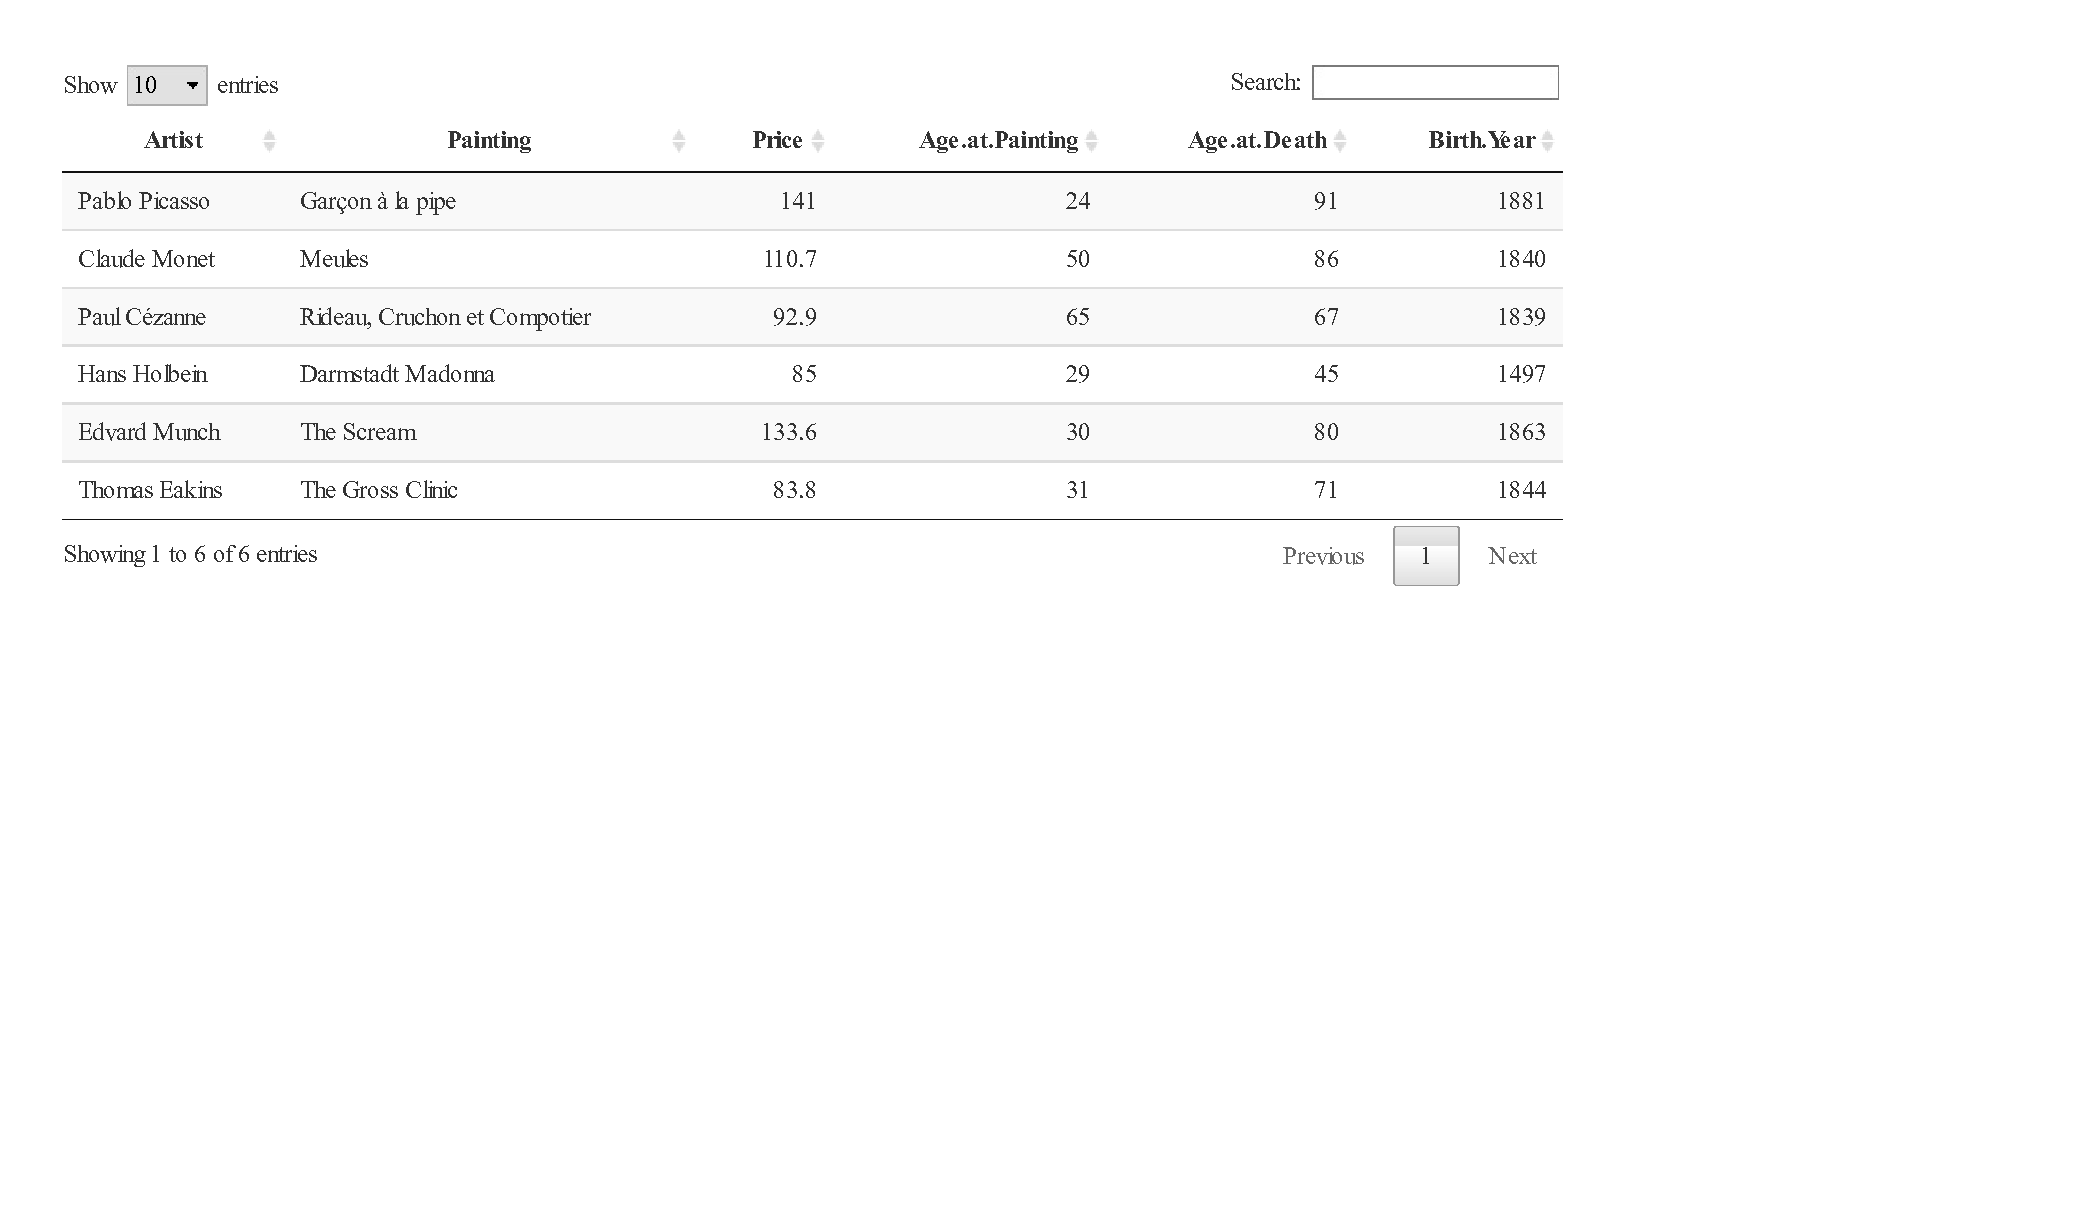
\includegraphics{Empirical-Research_files/figure-latex/unnamed-chunk-3-1.pdf}

\begin{infobox}warning

\textbf{Tabular data} is\ldots{}

common in data analysis. You can create a table in Word or Excel.

\end{infobox}

\hypertarget{data-in-a-graph}{%
\subsection{Data in a graph}\label{data-in-a-graph}}

Two variables from our data table can be depicted in what is called a \textbf{scatterplot}.

\begin{center}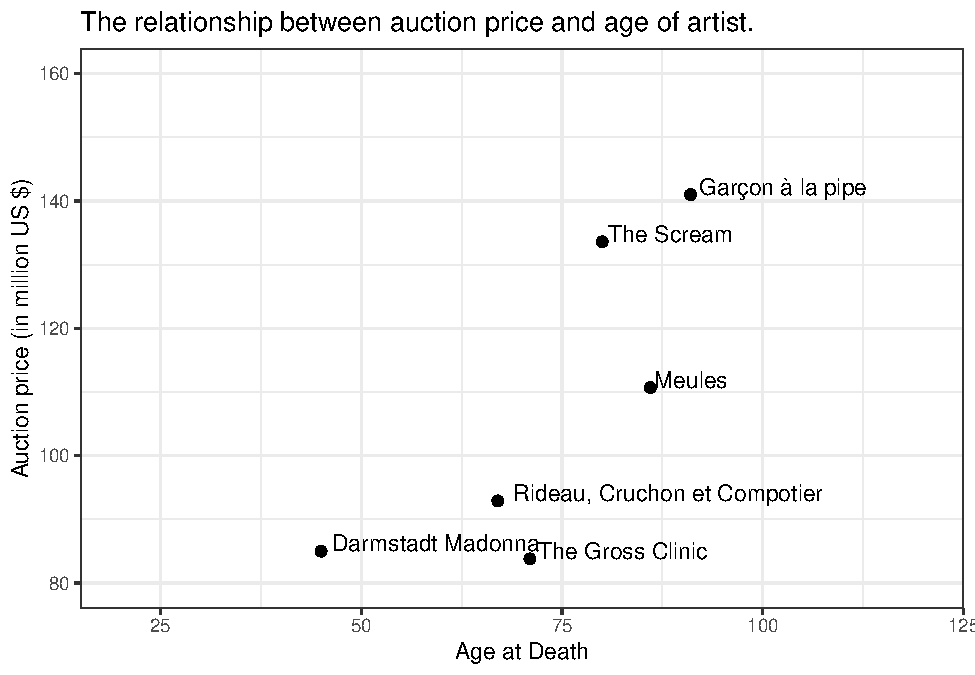
\includegraphics{Empirical-Research_files/figure-latex/unnamed-chunk-5-1} \end{center}

\begin{infobox}warning

\textbf{The axes are called} \ldots{}

\textbf{ordinate} or \textbf{y-axis} (here: price) and \textbf{abscicca} or \textbf{x-axis} (here: age).

\end{infobox}

\hypertarget{the-trend}{%
\subsection{The trend}\label{the-trend}}

\begin{infobox}warning
Can you spot a trend in the data?

\end{infobox}

The line plot suggests that the relationship between price and age exhibits a \textbf{positive trend}. There is an \textbf{increase} in price for older artists. The older the artist, the higher the auction prices.

\begin{center}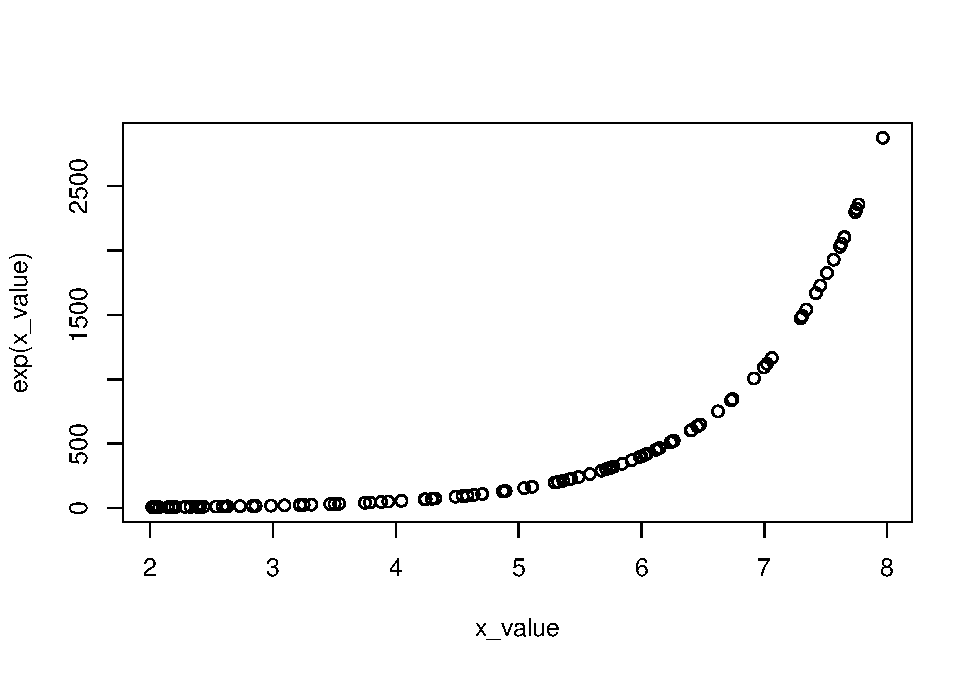
\includegraphics{Empirical-Research_files/figure-latex/unnamed-chunk-6-1} \end{center}

\hypertarget{the-blackbox}{%
\subsection{The blackbox}\label{the-blackbox}}

The mission is to find a mathematical function that describes the trend. In other words, we are looking for the black box that transforms the input into the output:


\includegraphics{function-fx-x2.svg}

\begin{infobox}warning

A \textbf{mathematical function} is \ldots{}

an expression, rule, or law that defines a relationship between one variable (the \textbf{independent variable}, on the x-axis) and another variable (the \textbf{dependent variable}, on the y-axis).

\end{infobox}

From looking at the graph, here are two suggestions:

\[ \begin{align}
\text{price} = 80 + 0.5 \cdot \text{age} \tag{Suggestion 1} \\
\text{price} = 90 + 0.2 \cdot \text{age} \tag{Suggestion 2} \\
\end{align}\]

\begin{infobox}warning

A \textbf{linear function} is \ldots{}

defined by two components, \textbf{intercept} (with the y-axis) and it's \textbf{slope}.

\end{infobox}

\begin{center}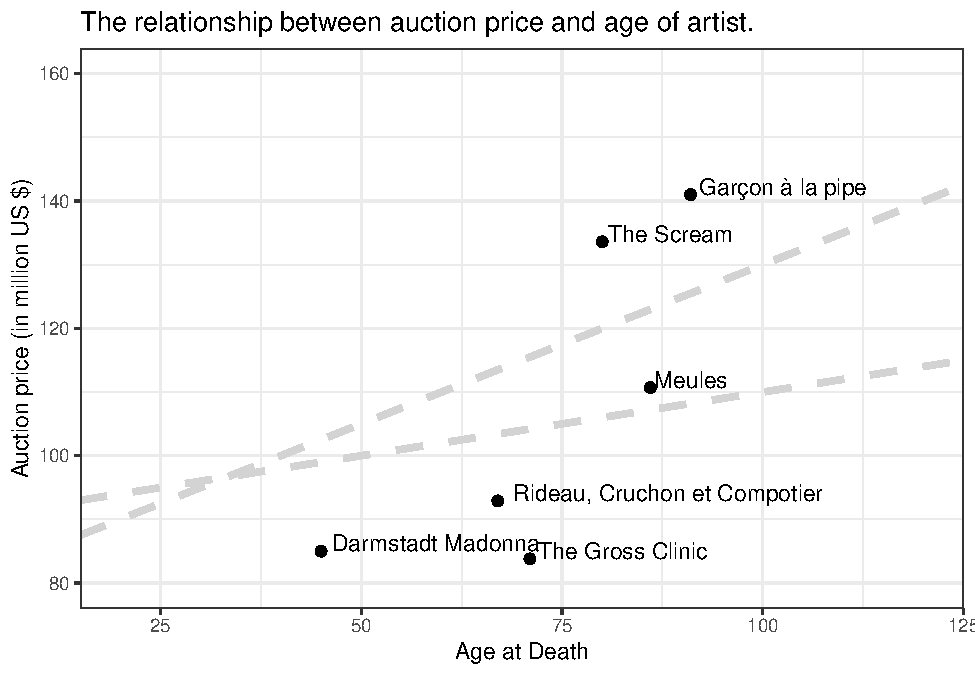
\includegraphics{Empirical-Research_files/figure-latex/unnamed-chunk-7-1} \end{center}

\begin{infobox}warning
How can we compare the two suggested lines? Which linear function represents the relationship best?

\end{infobox}

\hypertarget{nobodys-perfect}{%
\subsection{Nobody's perfect}\label{nobodys-perfect}}

We all make mistakes. So do the linear functions:

\[ \begin{align}
\text{price} = 80 + 0.5 \cdot \text{age} \tag{Suggestion 1} \\
101 = 80 + 0.5 \cdot 42 \tag{Calculation for Hohlbein} \\
\end{align}\]

The equation tells (or predicts) that for any artist at the age of 42 it expects a auction price for a painting of 101 million US Dollar. Darmstadt Madonna was sold for 85 million US dollar. The linear function overestimated the true value. When you look at the graph, you see some predictions are more accurate (close to the true values) than others. All are either above or below the line.

\begin{infobox}warning

A \textbf{residual} (or error) is \ldots{}

the vertical distance between the actual and the predicted value.

\end{infobox}

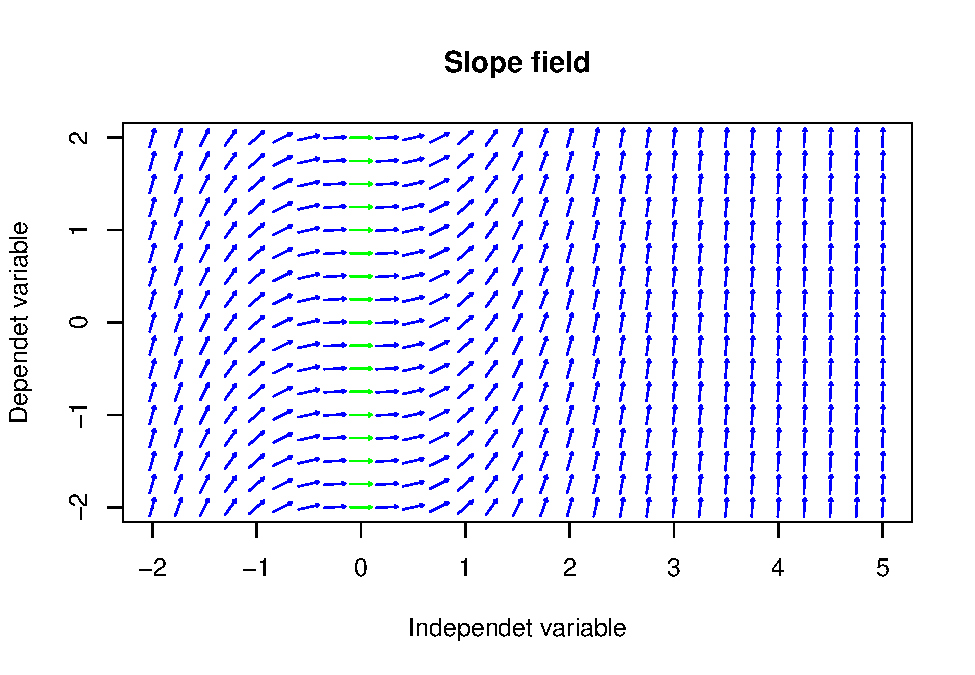
\includegraphics{Empirical-Research_files/figure-latex/unnamed-chunk-8-1.pdf}

\hypertarget{vocab-wrap-up}{%
\subsection{Vocab Wrap-Up}\label{vocab-wrap-up}}

Let's wrap up our regression vocab! We want to find an equation that describes the phenomenon of interest:

\[ \begin{align}
\text{outcome} &= f(\text{explanatory}) + \text{noise} \tag{Generic statistical model} \\
\text{outcome} &= \text{intercept} + \text{slope} \cdot \text{explanatory} + \text{noise} \tag{Generic linear model} \\
\end{align}\]

A \textbf{regression model} is suggested by the researcher. A more concrete regression model looks like this:

\[Y = \beta_1 + \beta_2 X + \epsilon\]

A model can be easy or complicated. It definitely contains variables and parameters.

\begin{itemize}
\tightlist
\item
  \textbf{Variables}: Things that we measure (or have data).
\item
  \textbf{Parameters}: Constant values we believe to represent some fundamental truth about the relationship between the variables.
\end{itemize}

What we (i.e.~the statistical software) actual do is an \textbf{estimation}. In textbooks the same equation can be found with hats:

\[   \widehat{Y}  = \widehat{\beta}_1 + \widehat{\beta}_2 \cdot X \]
\(\widehat{Y}\) are called the \textbf{fitted or predicted} values. \(\widehat{\beta}\) are \textbf{regression coefficients} (this is the estimate of the unknown population parameter). As we have seen in the graph before, the differences between the actual and the predicted values are the residuals \(e = Y - \widehat{Y}\).

\hypertarget{for-the-truly-dedicated}{%
\section{For the truly dedicated}\label{for-the-truly-dedicated}}

\begin{infobox}warning

Now we have all the ingredients we need.

\emph{Let's get this party started!}

\includegraphics{https://media1.tenor.com/images/6519b006f53708454922375a82c23682/tenor.gif?itemid=15161860}

\end{infobox}

The overall goal is to make as little as possible mistakes! What kind of mistake? The deviation from the observed values! What could come to your mind is to \textbf{minimize the sum of all errors}:

\[\sum e \rightarrow \min\]
But wait, there is more. Is it fair to say that the sum should be small? Compare \textbf{The Scream} and \textbf{Meules}, their deviations are \(+17.5\) and \(-13.6\) (very similar). So taken these two together, there's almost not mistake! That is to say, positive and negative deviations cancel each other out. Thus we need one more twist in the story:

\[\sum e^2 \rightarrow \min\]

\begin{infobox}warning

The fitting procedure is \ldots{}

is called \textbf{ordinary least squares} (short OLS). The goal of OLS is to \textbf{minimize the residual sum of squares}.

\end{infobox}

\hypertarget{algebra}{%
\subsection{Algebra}\label{algebra}}

\begin{infobox}warning
Algebra comes from Arabic, meaning ``reunion of broken parts''. We often work with matrices and vectors.

\end{infobox}

Now let's put all the things together. By convention, the \emph{normal} version of a vector is a vertical list of numbers in big parentheses (column vector). Transpose is when we change the rows and columns. In order to square a vector we need the following:

\[\sum e^2 = e^T \cdot e \rightarrow \min\]
Let's introduce matrix notation (there are 6 observations and two parameters):

\[ \begin{align}
Y &= \beta_0 + \beta_1 X + \epsilon \tag{X is a variable, Y is a variable} \\
\begin{pmatrix} Y_1 \\ Y_2 \\ Y_3 \\ Y_5 \\ Y_6 \end{pmatrix} &= \begin{pmatrix} 1 & X_{11} \\ 1 & X_{12} \\ 1 & X_{13} \\ 1 & X_{14} \\ 1 & X_{15} \\ 1 & X_{16}   \end{pmatrix} \begin{pmatrix} \beta_1 \\ \beta_2 \end{pmatrix} + \begin{pmatrix} \epsilon_1 \\ \epsilon_2 \\ \epsilon_3 \\ \epsilon_4 \\ \epsilon_5 \\ \epsilon_6 \\ \end{pmatrix} \\
y &= X \beta + \epsilon \tag{X is a matrix, y is a vector}
\end{align}\]

The residual is \(e = y - X \beta\) which we can plug in our minimal sum of squares:

\[\begin{align}
    \sum e^2 &= e^T \cdot e \tag{short RSS}\\
    &= (y - X \beta )^T (y - X \beta) \tag{$(A+B)^T = A^T + B^T$}\\
    &= (y^T - X^T \beta^T) (y - X \beta) \\
    &= y^T y - y^T X \beta - X^T \beta^T y + X^T \beta^T X \beta \\
    &= y^2 \underbrace{- 2 \beta^T X^T y}_{??} + \beta^2 X^2  \\
\end{align}\]

Did you notice what happened in the middle? The transpose of the first term is equal to the second:

\[\begin{align}
    (y^T X \beta)^T = y X^T \beta^T
\end{align}\]

\hypertarget{analysis}{%
\subsection{Analysis}\label{analysis}}

\begin{infobox}warning
In Analysis we often work with functions.

\end{infobox}

Next, we are ready to \textbf{optimize}. Optimization (in math and economics) is done by \textbf{differentiation}:

\[\begin{align}
    \frac{\partial RSS}{\partial \beta} &= -2 X^T y + 2 \beta X^T X = 0 \tag{first derivative equal to zero} \\
    2 \beta X^T X &= 2 X^T y \tag{rearrange terms}\\
    \beta X^T X &= X^T y \tag{the "normal equation"} \\
    \beta &= (X^T X)^{-1} X^T y \tag{Bam}\\
\end{align}\]

\hypertarget{take-the-long-way-home}{%
\subsection{Take the Long Way Home}\label{take-the-long-way-home}}

\begin{infobox}warning

\emph{The computer does the magic for us.}

\includegraphics{https://thumbs.gfycat.com/RemorsefulFairIndianpangolin-max-1mb.gif}

\end{infobox}

Those \(\beta\) coefficients are one of the most important regression results. Retrieve them step by step to enhance your understanding of the math and coding as the same time:

First, we retrieve matrix \texttt{X} from the data set:

\begin{Shaded}
\begin{Highlighting}[]
\NormalTok{X}
\end{Highlighting}
\end{Shaded}

\begin{verbatim}
##      [,1] [,2]
## [1,]    1   91
## [2,]    1   86
## [3,]    1   67
## [4,]    1   45
## [5,]    1   80
## [6,]    1   71
\end{verbatim}

Second, the transpose of \texttt{X} has two rows and six columns:

\begin{Shaded}
\begin{Highlighting}[]
\FunctionTok{t}\NormalTok{(X)}
\end{Highlighting}
\end{Shaded}

\begin{verbatim}
##      [,1] [,2] [,3] [,4] [,5] [,6]
## [1,]    1    1    1    1    1    1
## [2,]   91   86   67   45   80   71
\end{verbatim}

Next, calculate the square of the matrix (transpose times original):

\begin{Shaded}
\begin{Highlighting}[]
\FunctionTok{t}\NormalTok{(X)}\SpecialCharTok{\%*\%}\NormalTok{X}
\end{Highlighting}
\end{Shaded}

\begin{verbatim}
##      [,1]  [,2]
## [1,]    6   440
## [2,]  440 33632
\end{verbatim}

Then, the inverse of everything in parentheses (the above matrix product):

\begin{Shaded}
\begin{Highlighting}[]
\FunctionTok{solve}\NormalTok{(}\FunctionTok{t}\NormalTok{(X)}\SpecialCharTok{\%*\%}\NormalTok{X)}
\end{Highlighting}
\end{Shaded}

\begin{verbatim}
##             [,1]          [,2]
## [1,]  4.10546875 -0.0537109375
## [2,] -0.05371094  0.0007324219
\end{verbatim}

Next, the product of this inverse and the transpose:

\begin{Shaded}
\begin{Highlighting}[]
\FunctionTok{solve}\NormalTok{(}\FunctionTok{t}\NormalTok{(X)}\SpecialCharTok{\%*\%}\NormalTok{X) }\SpecialCharTok{\%*\%} \FunctionTok{t}\NormalTok{(X)}
\end{Highlighting}
\end{Shaded}

\begin{verbatim}
##             [,1]         [,2]         [,3]        [,4]         [,5]
## [1,] -0.78222656 -0.513671875  0.506835938  1.68847656 -0.191406250
## [2,]  0.01293945  0.009277344 -0.004638672 -0.02075195  0.004882813
##              [,6]
## [1,]  0.291992188
## [2,] -0.001708984
\end{verbatim}

Finally, we multiply the vector \(y\):

\begin{Shaded}
\begin{Highlighting}[]
\FunctionTok{solve}\NormalTok{(}\FunctionTok{t}\NormalTok{(X)}\SpecialCharTok{\%*\%}\NormalTok{X) }\SpecialCharTok{\%*\%} \FunctionTok{t}\NormalTok{(X) }\SpecialCharTok{\%*\%}\NormalTok{ y}
\end{Highlighting}
\end{Shaded}

\begin{verbatim}
##           [,1]
## [1,] 22.345215
## [2,]  1.165747
\end{verbatim}

There are two numbers. It's the \(\beta\) vector! The first entry is the \textbf{intercept} and the second is the \textbf{slope} of the linear function:

\[Price = 22.3452 + 1.1657 \cdot Age\]

\hypertarget{survival-of-the-fittest-line}{%
\section{Survival of the Fittest Line}\label{survival-of-the-fittest-line}}

\begin{infobox}warning
The above equation is the linear function that best describes the given data.

\end{infobox}

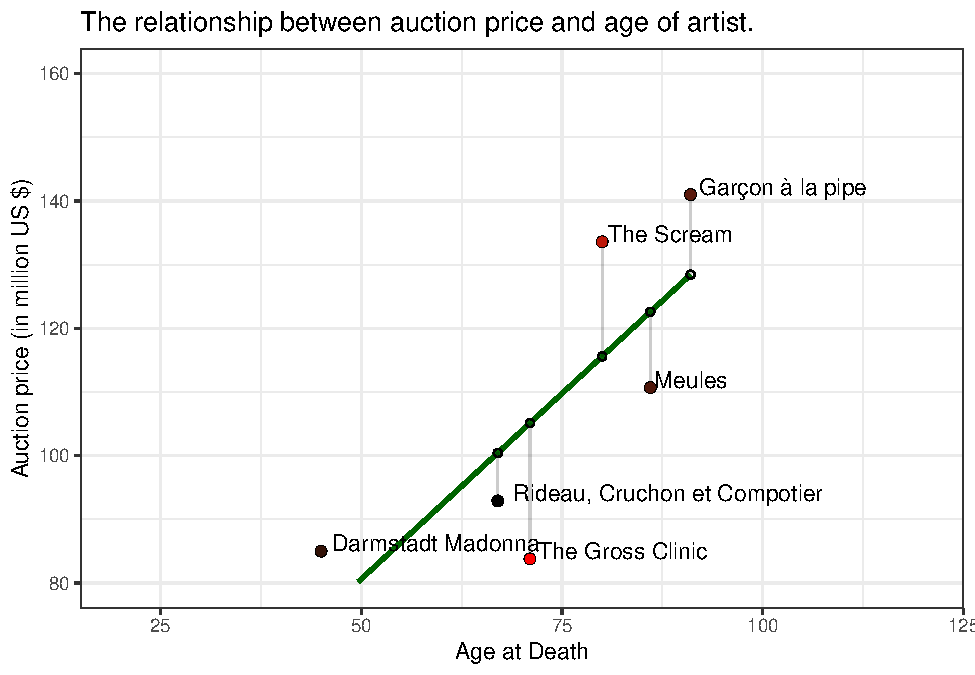
\includegraphics{Empirical-Research_files/figure-latex/unnamed-chunk-16-1.pdf}

\hypertarget{on-the-shoulders-of-giants}{%
\section{On the Shoulders of Giants}\label{on-the-shoulders-of-giants}}

Fortunately, we are \href{https://en.wikipedia.org/wiki/Standing_on_the_shoulders_of_giants}{standing on the shoulders of giants}. Clever people implemented the linear regression and all kinds of regressions and statistical tests in R.

\begin{Shaded}
\begin{Highlighting}[]
\FunctionTok{lm}\NormalTok{(Price }\SpecialCharTok{\textasciitilde{}}\NormalTok{ Age.at.Death, }\AttributeTok{data =}\NormalTok{ artists)}
\end{Highlighting}
\end{Shaded}

\begin{verbatim}
## 
## Call:
## lm(formula = Price ~ Age.at.Death, data = artists)
## 
## Coefficients:
##  (Intercept)  Age.at.Death  
##       22.345         1.166
\end{verbatim}

But this would have been less fun!

\begin{infobox}warning

\emph{That's all folks! }

\includegraphics{https://static.wikia.nocookie.net/looneytunes/images/e/e1/All.jpg/revision/latest/scale-to-width-down/1000?cb=20150313020828}

\end{infobox}

\hypertarget{methods}{%
\chapter{Methods}\label{methods}}

We describe our methods in this chapter.

\hypertarget{slope-fields}{%
\chapter{Slope Fields}\label{slope-fields}}

\hypertarget{definition}{%
\section{Definition}\label{definition}}

\begin{quote}
Slope fields (also called direction fields) are a graphical representation of the solutions to a first-order differential equation of a scalar function. Solutions to a slope field are functions drawn as solid curves. A slope field shows the slope of a differential equation at certain vertical and horizontal intervals on the x-y plane, and can be used to determine the approximate tangent slope at a point on a curve, where the curve is some solution to the differential equation.

\hfill Wikipedia contributors. (2021, May 17). Slope field. In Wikipedia, The Free Encyclopedia. Retrieved 05:51, June 16, 2021, from \url{https://en.wikipedia.org/w/index.php?title=Slope_field\&oldid=1023635282}
\end{quote}

\hypertarget{slope-fields-in-r}{%
\section{Slope Fields in R}\label{slope-fields-in-r}}

There's no need to build everything from scratch. This original post \url{https://www.r-bloggers.com/2014/09/generate-slope-fields-in-r-and-python/} has been put into a \texttt{SlopeField} function here \url{https://stackoverflow.com/questions/47984874/how-to-create-a-slope-field-in-r}.

Show me the code.

\begin{Shaded}
\begin{Highlighting}[]
\NormalTok{SlopeField }\OtherTok{=} \ControlFlowTok{function}\NormalTok{(FUN,}\AttributeTok{xi =} \SpecialCharTok{{-}}\DecValTok{5}\NormalTok{,}\AttributeTok{xs =} \DecValTok{5}\NormalTok{,}\AttributeTok{yi =} \SpecialCharTok{{-}}\DecValTok{5}\NormalTok{,}\AttributeTok{ys =} \DecValTok{5}\NormalTok{, }\AttributeTok{radius =} \FloatTok{0.1}\NormalTok{, }\AttributeTok{grid.by =} \FloatTok{0.25}\NormalTok{)\{}
  \CommentTok{\# FUN   {-} given function ODE i.e:  }
  \CommentTok{\# xi,xs {-} lower and upper bound {-} x {-} plot}
  \CommentTok{\# yi,ys {-} lower and upper bound {-} y {-} plot}
  
  \CommentTok{\# grid points}
\NormalTok{  seqx }\OtherTok{=} \FunctionTok{seq}\NormalTok{(xi,xs,grid.by)}
\NormalTok{  seqy }\OtherTok{=} \FunctionTok{seq}\NormalTok{(yi,ys,grid.by)}
  
  \CommentTok{\# plot}
\NormalTok{  f }\OtherTok{=} \FunctionTok{c}\NormalTok{(xi,xs) }
\NormalTok{  h }\OtherTok{=} \FunctionTok{c}\NormalTok{(yi,ys)}
  \FunctionTok{plot}\NormalTok{(f,h,}\AttributeTok{main=}\StringTok{"Slope field"}\NormalTok{, }\AttributeTok{ylab =} \StringTok{"Dependet variable"}\NormalTok{, }\AttributeTok{xlab =} \StringTok{"Independet variable"}\NormalTok{, }\AttributeTok{pch =} \StringTok{"."}\NormalTok{)}
  
  \CommentTok{\# arrows}
  
  \ControlFlowTok{for}\NormalTok{(x }\ControlFlowTok{in}\NormalTok{ seqx)\{}
    \ControlFlowTok{for}\NormalTok{(y }\ControlFlowTok{in}\NormalTok{ seqy)\{}
\NormalTok{      ym }\OtherTok{=}\NormalTok{ y}
\NormalTok{      xm }\OtherTok{=}\NormalTok{ x}
      
\NormalTok{      slope }\OtherTok{=} \FunctionTok{unlist}\NormalTok{(}\FunctionTok{FUN}\NormalTok{(x,y))}
      
      \ControlFlowTok{if}\NormalTok{(}\FunctionTok{is.na}\NormalTok{(slope))\{}
\NormalTok{        cor }\OtherTok{=} \StringTok{"black"}
\NormalTok{      \} }\ControlFlowTok{else} \ControlFlowTok{if}\NormalTok{(slope }\SpecialCharTok{\textgreater{}} \DecValTok{0}\NormalTok{)\{}
\NormalTok{        cor }\OtherTok{=} \StringTok{"blue"}
\NormalTok{      \}}\ControlFlowTok{else} \ControlFlowTok{if}\NormalTok{ (slope }\SpecialCharTok{\textless{}} \DecValTok{0}\NormalTok{) \{}
\NormalTok{        cor }\OtherTok{=} \StringTok{"red"}
\NormalTok{      \}}\ControlFlowTok{else} \ControlFlowTok{if}\NormalTok{(slope }\SpecialCharTok{==} \DecValTok{0}\NormalTok{) \{}
\NormalTok{        cor }\OtherTok{=} \StringTok{"green"}
\NormalTok{      \}}
      \FunctionTok{arrows}\NormalTok{(radius}\SpecialCharTok{*}\FunctionTok{cos}\NormalTok{(}\FunctionTok{atan}\NormalTok{(slope)}\SpecialCharTok{+}\NormalTok{pi)}\SpecialCharTok{+}\NormalTok{xm,}
\NormalTok{             radius}\SpecialCharTok{*}\FunctionTok{sin}\NormalTok{(}\FunctionTok{atan}\NormalTok{(slope)}\SpecialCharTok{+}\NormalTok{pi)}\SpecialCharTok{+}\NormalTok{ym,}
\NormalTok{             radius}\SpecialCharTok{*}\FunctionTok{cos}\NormalTok{(}\FunctionTok{atan}\NormalTok{(slope))}\SpecialCharTok{+}\NormalTok{xm,}
\NormalTok{             radius}\SpecialCharTok{*}\FunctionTok{sin}\NormalTok{(}\FunctionTok{atan}\NormalTok{(slope))}\SpecialCharTok{+}\NormalTok{ym, }
             \AttributeTok{length =} \FloatTok{0.2}\SpecialCharTok{*}\NormalTok{radius, }\AttributeTok{col=}\NormalTok{ cor)}
\NormalTok{    \}}
\NormalTok{  \}}
\NormalTok{\}}
\end{Highlighting}
\end{Shaded}

We can specify an ODE in another function and plot its slope field. The suggested example is

\[y'(t) = y^2 - t \]

\begin{Shaded}
\begin{Highlighting}[]
\NormalTok{ode }\OtherTok{=} \ControlFlowTok{function}\NormalTok{(t, y)\{}
\NormalTok{  dydt }\OtherTok{\textless{}{-}}\NormalTok{ y}\SpecialCharTok{\^{}}\DecValTok{2}\SpecialCharTok{{-}}\NormalTok{t}
  \FunctionTok{list}\NormalTok{(dydt)}
\NormalTok{\}}
\end{Highlighting}
\end{Shaded}

Let's draw the slope field.

\begin{Shaded}
\begin{Highlighting}[]
\FunctionTok{SlopeField}\NormalTok{(ode, }\AttributeTok{xi =} \SpecialCharTok{{-}}\DecValTok{2}\NormalTok{, }\AttributeTok{xs =} \DecValTok{5}\NormalTok{, }\AttributeTok{yi =} \SpecialCharTok{{-}}\DecValTok{2}\NormalTok{, }\AttributeTok{ys =} \DecValTok{2}\NormalTok{,}\AttributeTok{radius =} \FloatTok{0.1}\NormalTok{, }\AttributeTok{grid.by =} \FloatTok{0.25}\NormalTok{)}
\end{Highlighting}
\end{Shaded}

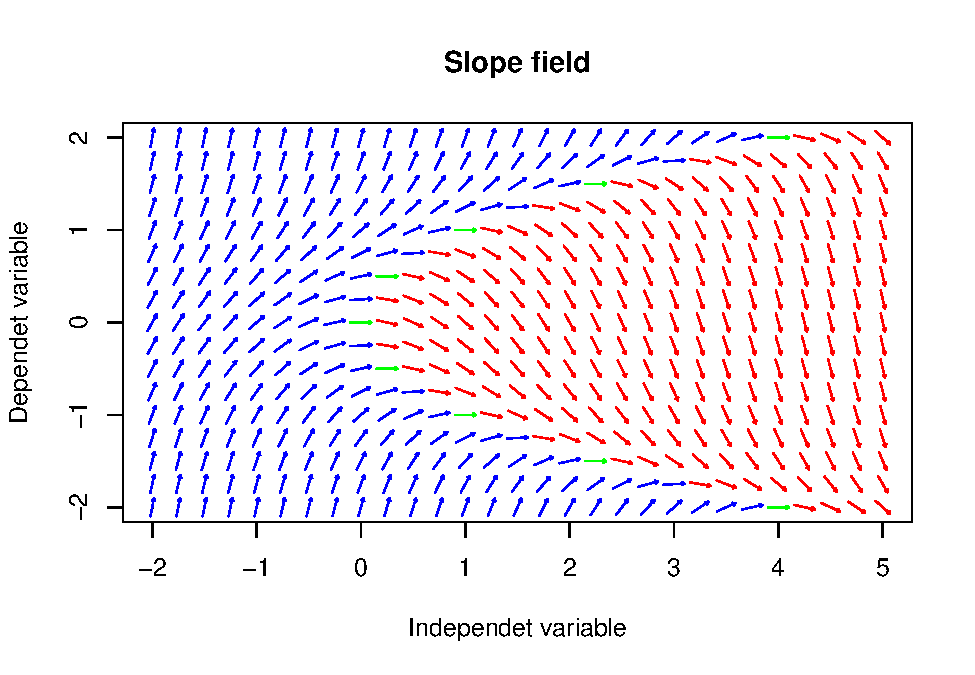
\includegraphics{Empirical-Research_files/figure-latex/unnamed-chunk-20-1.pdf}

The graph looks nice and interesting. But can how can we get the ODE solution from this graph? Can you spot the slip in the code and graph?

\hypertarget{understandable-examples}{%
\section{Understandable Examples}\label{understandable-examples}}

\hypertarget{y-y}{%
\subsection{y' = y}\label{y-y}}

Even without a background in differential equations, think about the following:

\[y'(x) = y(x)\]
We are looking for a function \(y(x)\) that is identical to its first derivative \(y'(x)\). Perhaps you remember such a function from your last math class (analysis). It is the exponential function, that basically does not change by differentiation.

\[y(x) = e^x \Rightarrow y'(x) = e^x \]

\begin{Shaded}
\begin{Highlighting}[]
\NormalTok{ode\_1 }\OtherTok{=} \ControlFlowTok{function}\NormalTok{(t, y)\{}
\NormalTok{  dydt }\OtherTok{\textless{}{-}}\NormalTok{ y}
  \FunctionTok{list}\NormalTok{(dydt)}
\NormalTok{\}}

\FunctionTok{SlopeField}\NormalTok{(ode\_1, }\AttributeTok{xi =} \SpecialCharTok{{-}}\DecValTok{2}\NormalTok{, }\AttributeTok{xs =} \DecValTok{5}\NormalTok{, }\AttributeTok{yi =} \SpecialCharTok{{-}}\DecValTok{2}\NormalTok{, }\AttributeTok{ys =} \DecValTok{2}\NormalTok{,}\AttributeTok{radius =} \FloatTok{0.1}\NormalTok{, }\AttributeTok{grid.by =} \FloatTok{0.25}\NormalTok{)}
\end{Highlighting}
\end{Shaded}

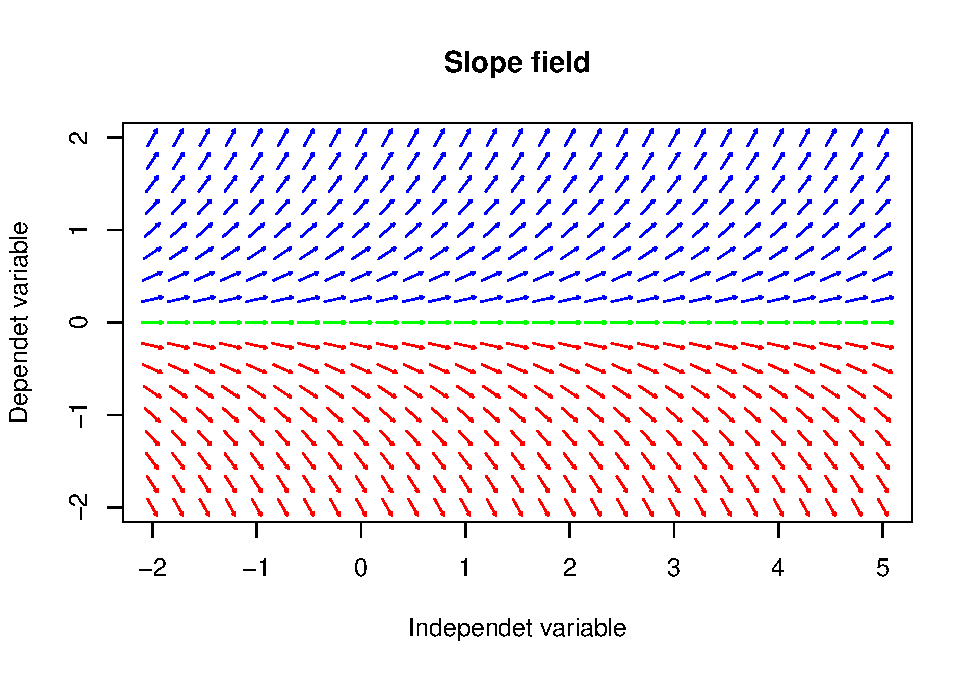
\includegraphics{Empirical-Research_files/figure-latex/unnamed-chunk-21-1.pdf}

Can you see something like the exponential function in this slope field?

Show me how an exponential function looks like.

\begin{Shaded}
\begin{Highlighting}[]
\NormalTok{x\_value}\OtherTok{\textless{}{-}}\FunctionTok{runif}\NormalTok{(}\DecValTok{100}\NormalTok{,}\DecValTok{2}\NormalTok{,}\DecValTok{8}\NormalTok{)}
\FunctionTok{plot}\NormalTok{(x\_value,}\FunctionTok{exp}\NormalTok{(x\_value))}
\end{Highlighting}
\end{Shaded}

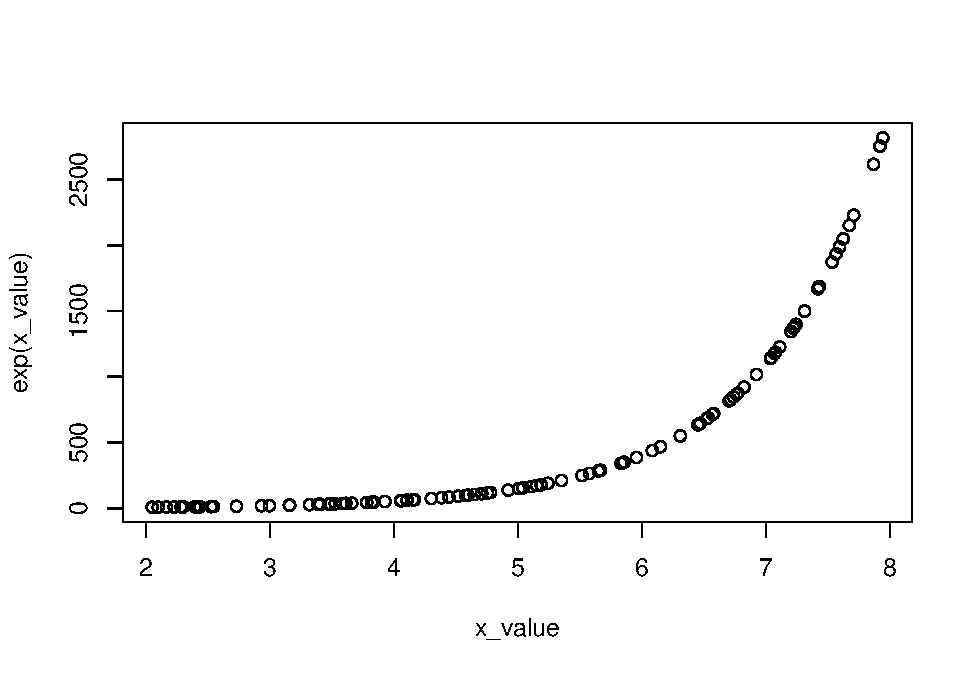
\includegraphics{Empirical-Research_files/figure-latex/unnamed-chunk-22-1.pdf}

Perhaps you can spot something like the \(y(x) = e^x\) in the blue area. But how about the red arrows? Any mirror at the x-axis is also a valid solution to the problem. How do we mirror? Use a factor in front of the e function. This may be negative.

\[y(x) = C \cdot e^x \Rightarrow y'(x) = C \cdot e^x \]

\hypertarget{y--y}{%
\subsection{y' = -y}\label{y--y}}

Let's give it another try. Which function equals its first derivative (after changing sign).

\[y'(x) = -y(x)\]

It is a sibling of the \(e^x\). The solution is \(y(x) = C \cdot e^{-x}\).

\begin{Shaded}
\begin{Highlighting}[]
\NormalTok{ode\_2 }\OtherTok{=} \ControlFlowTok{function}\NormalTok{(t, y)\{}
\NormalTok{  dydt }\OtherTok{\textless{}{-}} \SpecialCharTok{{-}}\NormalTok{y}
  \FunctionTok{list}\NormalTok{(dydt)}
\NormalTok{\}}

\FunctionTok{SlopeField}\NormalTok{(ode\_2, }\AttributeTok{xi =} \SpecialCharTok{{-}}\DecValTok{2}\NormalTok{, }\AttributeTok{xs =} \DecValTok{5}\NormalTok{, }\AttributeTok{yi =} \SpecialCharTok{{-}}\DecValTok{2}\NormalTok{, }\AttributeTok{ys =} \DecValTok{2}\NormalTok{,}\AttributeTok{radius =} \FloatTok{0.1}\NormalTok{, }\AttributeTok{grid.by =} \FloatTok{0.25}\NormalTok{)}
\end{Highlighting}
\end{Shaded}

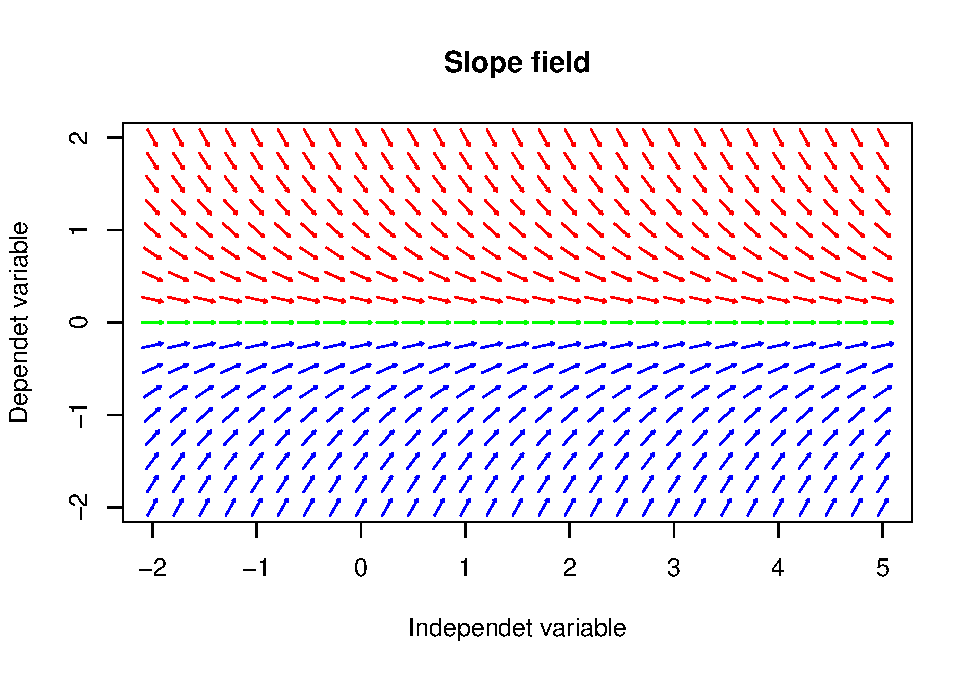
\includegraphics{Empirical-Research_files/figure-latex/unnamed-chunk-23-1.pdf}

\hypertarget{y-x2}{%
\subsection{y' = x\^{}2}\label{y-x2}}

Wait, there's no more y on the RHS. Don't worry. That'll make it even easier. What is the integral of \(x^2\)? You may expect

\[y'(x) = x^2 \Rightarrow \int x^2 dx = 1/3 \cdot x^3 + C\]
Okay, the general shape is a cubic function. Can you spot a cubic function?

\begin{Shaded}
\begin{Highlighting}[]
\NormalTok{ode\_3 }\OtherTok{=} \ControlFlowTok{function}\NormalTok{(t, y)\{}
\NormalTok{  dydt }\OtherTok{\textless{}{-}}\NormalTok{ t}\SpecialCharTok{\^{}}\DecValTok{2}
  \FunctionTok{list}\NormalTok{(dydt)}
\NormalTok{\}}

\FunctionTok{SlopeField}\NormalTok{(ode\_3, }\AttributeTok{xi =} \SpecialCharTok{{-}}\DecValTok{2}\NormalTok{, }\AttributeTok{xs =} \DecValTok{5}\NormalTok{, }\AttributeTok{yi =} \SpecialCharTok{{-}}\DecValTok{2}\NormalTok{, }\AttributeTok{ys =} \DecValTok{2}\NormalTok{,}\AttributeTok{radius =} \FloatTok{0.1}\NormalTok{, }\AttributeTok{grid.by =} \FloatTok{0.25}\NormalTok{)}
\end{Highlighting}
\end{Shaded}

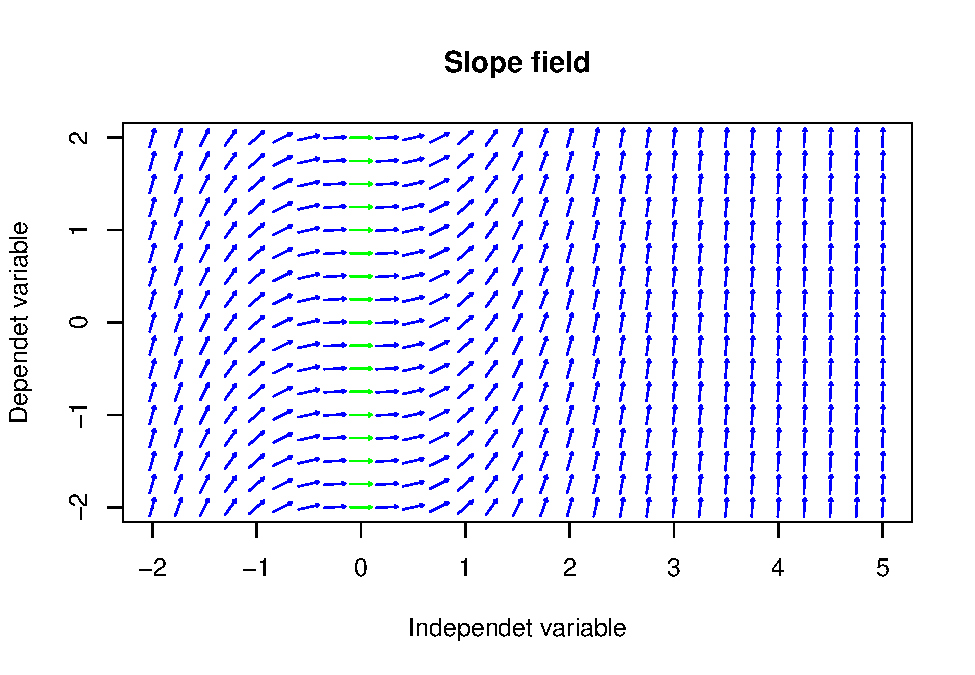
\includegraphics{Empirical-Research_files/figure-latex/unnamed-chunk-24-1.pdf}

\hypertarget{initial-value-problem}{%
\section{Initial value problem}\label{initial-value-problem}}

Recap, the prior solution was \(y(x) = 1/3 \cdot x^3 + C\). Due to \(C\) this is a family of curves. If we specify some of them, that's called the initial value problem. This \emph{problem} makes is actually even more easy to understand the slope field. Let's add two particular cubic functions for \(C = 0\) and \(C = 0.5\).

\begin{Shaded}
\begin{Highlighting}[]
\FunctionTok{SlopeField}\NormalTok{(ode\_3, }\AttributeTok{xi =} \SpecialCharTok{{-}}\DecValTok{2}\NormalTok{, }\AttributeTok{xs =} \DecValTok{5}\NormalTok{, }\AttributeTok{yi =} \SpecialCharTok{{-}}\DecValTok{2}\NormalTok{, }\AttributeTok{ys =} \DecValTok{2}\NormalTok{,}\AttributeTok{radius =} \FloatTok{0.1}\NormalTok{, }\AttributeTok{grid.by =} \FloatTok{0.25}\NormalTok{)}
\end{Highlighting}
\end{Shaded}

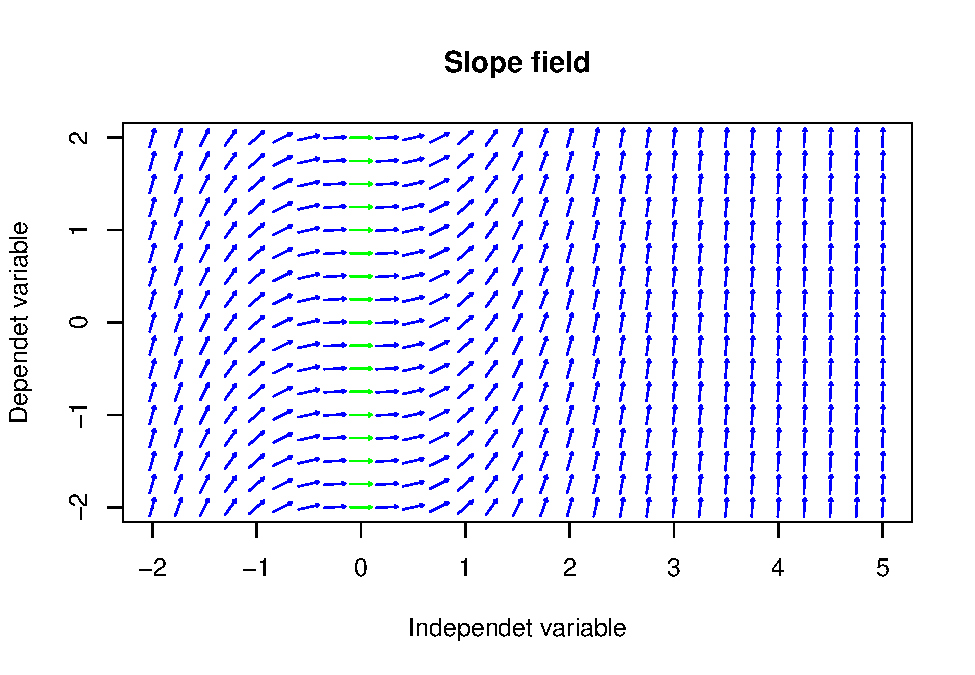
\includegraphics{Empirical-Research_files/figure-latex/unnamed-chunk-25-1.pdf}

\begin{Shaded}
\begin{Highlighting}[]
\CommentTok{\#lines(y,1/3*x*x*x,col="red", lwd=2)}
\CommentTok{\#lines(y,1/3*x*x*x+0.5,col="orange", lwd=2)}
\end{Highlighting}
\end{Shaded}

Enjoy. Learn. Share.

\hypertarget{git-and-github}{%
\chapter{Git and Github}\label{git-and-github}}

\hypertarget{install-github-and-git}{%
\section{Install Github and Git}\label{install-github-and-git}}

\begin{itemize}
\tightlist
\item
  Get RStudio \url{https://www.rstudio.com/products/rstudio/download/}
\item
  Get Github account \url{https://github.com/}
\item
  Set up Github pages \url{https://pages.github.com/}
\item
  Download Git \url{https://git-scm.com/}
\end{itemize}

Create a ``special repository'' for GitHub Pages. Only this can turn the branch into docs (1 for free).

\begin{itemize}
\tightlist
\item
  Repository: \url{https://github.com/MarcoKuehne/marcokuehne.github.io}
\item
  Homepage: \url{https://marcokuehne.github.io/}
\end{itemize}

Create (or re-open) your R project inside RStudio.

In R console use \texttt{usethis::use\_git()} which always gives three different answers in random order. Confirm accordingly.

\hypertarget{working-with-git}{%
\section{Working with Git}\label{working-with-git}}

Use the terminal inside RStudio. Copy paste into terminal with: \texttt{CTRL\ +\ SHIFT\ +\ V}.

\hypertarget{git-version}{%
\subsection{git version}\label{git-version}}

Let's start with commands that cannot do any harm (it's 2.32 in 08/2021):

\begin{verbatim}
git version
\end{verbatim}

\hypertarget{git-config}{%
\subsection{git config}\label{git-config}}

First, configure github user information on your system. Use the R builtin terminal:

\begin{verbatim}
git config --global user.email MAIL
git config --global user.name NAME
\end{verbatim}

Now, you can commit (upload) changes from RStudio to Github Pages. Check out \texttt{git\ config\ -\/-list}.

\hypertarget{git-init}{%
\subsection{git init}\label{git-init}}

Use \texttt{git\ init} to initialize the repository. It is used to create a new empty repository or directory consisting of files' with the hidden directory. `.git' is created at the top level of your project, which places all of the revision information in one place.

Show what is connected with:

\begin{verbatim}
git remote -v show
\end{verbatim}

\hypertarget{git-status-and-diff}{%
\subsection{git status and diff}\label{git-status-and-diff}}

Shows you which files are in this staging area, and which files have changes that haven't yet been put there. In order to compare the file as it currently is to what you last saved, you can use \texttt{git\ diff\ filename}, e.g.~\texttt{git\ diff\ README.md} in the terminal. \texttt{git\ diff} without any file names will show you all the changes in your repository, while git diff directory will show you the changes to the files in some directory.

\hypertarget{git-commit}{%
\subsection{git commit}\label{git-commit}}

To save the changes in the staging area, you use the command \texttt{git\ commit}. It always saves everything that is in the staging area as one unit: as you will see later, when you want to undo changes to a project, you undo all of a commit or none of it.

Commit requires a message (comment). How to write a good git commit \url{message:l}

\url{https://chris.beams.io/posts/git-commit/}

\hypertarget{git-add}{%
\subsection{git add}\label{git-add}}

\ldots{}

\hypertarget{git-remote-add}{%
\subsection{git remote add}\label{git-remote-add}}

I would like to have something like \texttt{git\ remote\ add\ ...} and \texttt{git\ push\ ...}, not working.

I can add and remove origins, don't know what it means: \texttt{git\ remote\ rm\ origin}

Use git add . in your bash to add all the files to the given folder.

Use git status in your bash to view all the files which are going to be staged to the first commit.

Create \textbf{git remote add}

git remote add origin \url{https://github.com/MarcoKuehne/marcokuehne.github.git}
git remote add origin \url{https://github.com/MarcoKuehne/marcokuehne.github.io}
git remote add origin \url{https://github.com/MarcoKuehne/marcokuehne.github.io.git}

git remote add \href{mailto:git@github.com}{\nolinkurl{git@github.com}}:/.git
git remote add \href{mailto:git@github.com}{\nolinkurl{git@github.com}}:MarcoKuehne/marcokuehne.github.git
git remote add \href{mailto:git@github.com}{\nolinkurl{git@github.com}}:MarcoKuehne/marcokuehne.github.io does not appear to be a repository
git remote add \href{mailto:git@github.com}{\nolinkurl{git@github.com}}:MarcoKuehne/marcokuehne.github.io.git combine both

\hypertarget{git-push}{%
\subsection{git push}\label{git-push}}

git push -u origin main
git push -u origin master
git push origin master
git push origin main
git push --set-upstream origin main
git push -f origin main \# worked somehow!!!

If positive, it asks for github credentials.

\url{https://www.datacamp.com/community/tutorials/git-push-pull}

\hypertarget{basic-routines}{%
\section{Basic Routines}\label{basic-routines}}

\hypertarget{add-commit-push}{%
\subsection{Add + Commit + Push}\label{add-commit-push}}

I make changes to any one of my markdown files, e.g.~the \texttt{README.md} (this can also be done via GitHub web interface) on my local machine. After notoriously saving this on my local machine (STRG+S) it appears in the \emph{stage area} in the right upper panel in RStudio. Commit and push can be either done in RStudio or via terminal line (also in RStudio).

First, let's do it via ``clicking''. Select the staged file. Click ``commit''. A new windows opens and displays the changes in your file. Write a new commit message of amend a previous commit. Click ``close''. From this additional window (or the right upper panel in RStudio) click the green push arrow. Hopefully it will say ``HEAD -\textgreater{} main''. Close. Done. The result should be available on your github repository immediately.

The same procedure via the terminal:

\begin{verbatim}
git add 05-git.Rmd
git commit -m "Updated the git short tutorial"
git push 
\end{verbatim}

How to push? Easy \ldots{}

I need to \texttt{pull} these changes into RStudio. Check the right upper panel ``Diff''. Select \texttt{pull}. You can also find big blue down and green up arrows.

I add this sentence. I save on RStudio, thus it appears as a change to \texttt{README.md} in the Git panel. I select this file and green up arrow (push). I enter my credentials and close (see \url{https://docs.github.com/en/get-started/getting-started-with-git/why-is-git-always-asking-for-my-password}). Here you might use a personal access token. I click \texttt{commit}, enter a commit message, click \texttt{commit} again and close the extra window.

\hypertarget{resources}{%
\section{Resources}\label{resources}}

You can start reading about bookdowns from the inventor:

\url{https://bookdown.org/yihui/bookdown/}

This is pretty advanced and I can't understand a tiny piece of it.

Another option is to start a repo and book by copying ``awesome book'' from another repo.

\url{https://jules32.github.io/bookdown-tutorial/setup.html}

This tutorial worked to push a book to a standard repo. But there were problem with the doc branch.

After I forgot how to start my project or where to find it, I checked:

\url{https://happygitwithr.com/rstudio-git-github.html\#make-local-changes-save-commit}

started a new project with my repo link and a new session. This forks or fetches or pulls or downloads the repo. Now I will try to re-upload the minimal change from today.

Another personal description can be found here:

\url{https://rachaellappan.github.io/bookdown/}

\begin{verbatim}
This enourmously helped with the understanding of commits and pushs on git:

<http://www.differencebetween.net/technology/difference-between-commit-and-push/>
\end{verbatim}

\begin{itemize}
\tightlist
\item
  \texttt{git\ commit\ -m\ "Started\ book"}
\end{itemize}

I followed the video ``How to create a bookdown book in 5 minutes'':

\url{https://www.youtube.com/watch?v=m5D-yoH416Y}

It did not work.

Explaining terminology:

\url{https://www.notion.so/zarkom/Introduction-to-Git-ac396a0697704709a12b6a0e545db049}

Learn Git in 15 Min:

\url{https://www.youtube.com/watch?v=USjZcfj8yxE}

Learn GitHub in 20 Min:

\url{https://www.youtube.com/watch?v=nhNq2kIvi9s}

\url{https://medium.com/@delucmat/how-to-publish-bookdown-projects-with-github-actions-on-github-pages-6e6aecc7331e}

  \bibliography{book.bib,packages.bib}

\end{document}
